\vspace{-5pt}
\section{Technical Overview}
\label{sec:overview}

In order to generate scanning trajectories, our algorithm leverages a coarse estimate of the scene geometry.
Initially, we do not have any estimate of the scene geometry, so we adopt an \emph{explore-then-exploit} approach.

In the \emph{explore} phase, we fly our drone (i.e., we command our drone to fly autonomously) along a default trajectory at a safe distance above the scene, acquiring a sequence of images as we are flying.
We land our drone, and subsequently feed the acquired images to an open-source multi-view stereo pipeline, thereby obtaining a coarse estimate of the scene geometry, and  a strictly conservative estimate of the scene's free space.
We include a more detailed discussion of our \emph{explore} phase in the supplementary material.

In the \emph{exploit} phase, we use this additional information about the scene to plan a scanning trajectory that attempts to maximize the fidelity of the resulting 3D reconstruction.
At the core of our planning algorithm, is a coverage model that accounts for the domain-specific requirements of multi-view stereo reconstruction (Section \ref{sec:coverage_model}).
Using this model, we generate a scanning trajectory that maximizes scene coverage, while respecting the drone's limited flight time (Section \ref{sec:trajectories}). 
We fly the drone along our scanning trajectory, acquiring another sequence of images.
Finally, we land our drone again, and we feed all the images we have acquired to our multi-view stereo pipeline to obtain a detailed 3D reconstruction of the scene.

\begin{figure}[t]
\begin{center}
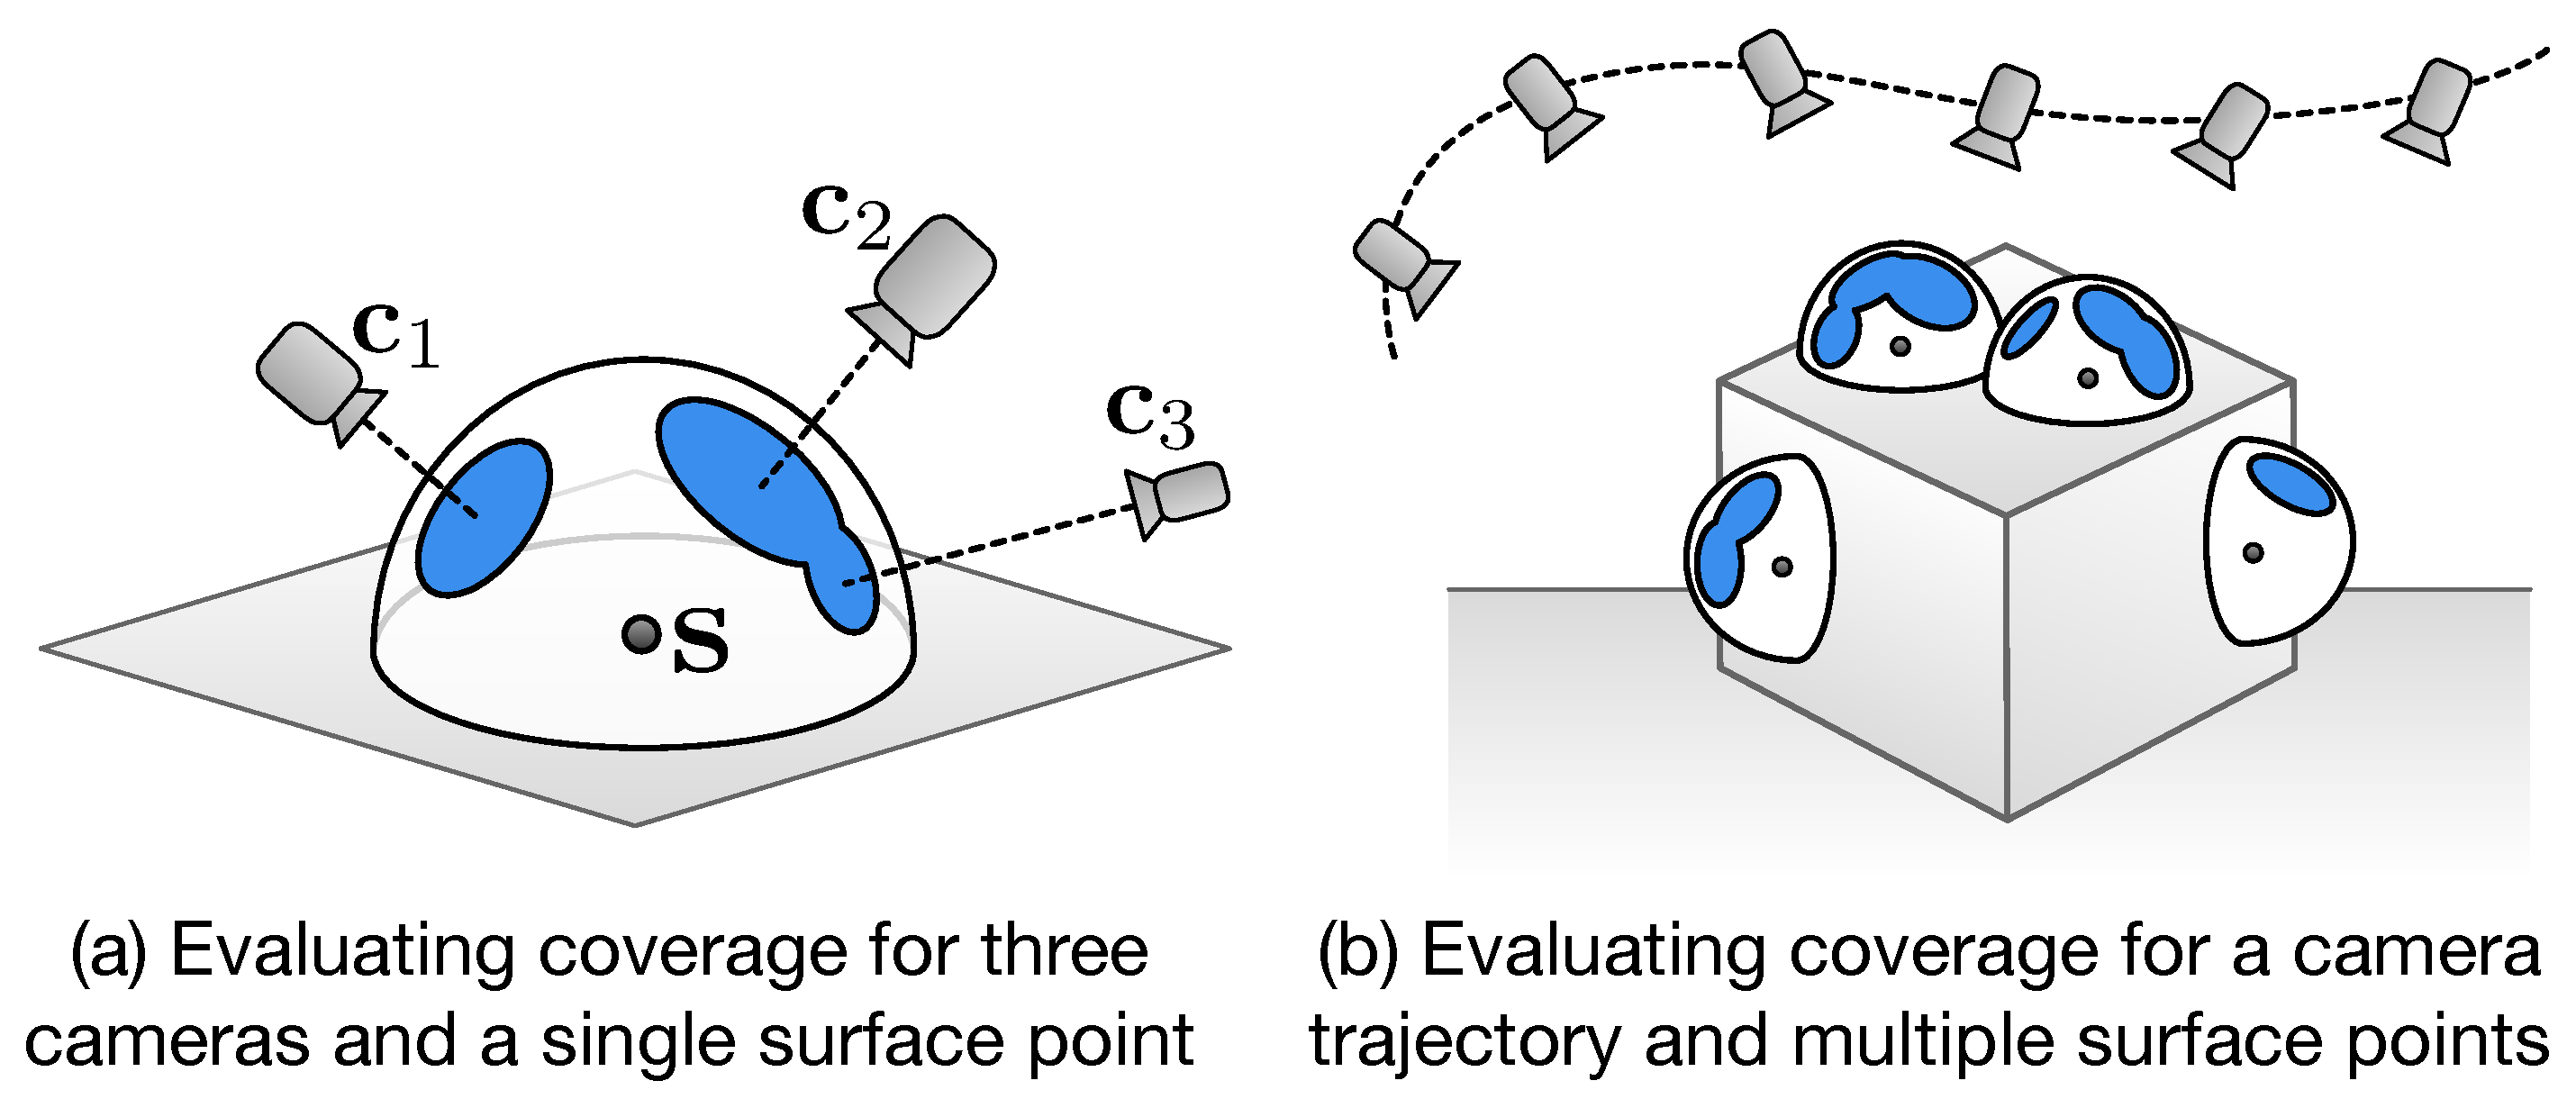
\includegraphics[width=0.47\textwidth]{images/2017_iccv/coverage_model_horizontal.pdf}{\vspace{-7pt}}
\end{center}
\caption{
Our coverage model for quantifying the usefulness of camera trajectories for multi-view stereo reconstruction. More useful trajectories cover more of the hemisphere of viewing angles around surface points.
(a) An illustrative example showing coverage of a single surface point with three cameras. Each camera covers a circular disk on a hemisphere around the surface point $\mathbf{s}$, and the total solid angle covered by all the disks determines the total usefulness of the cameras.
Note that the angular separation (i.e., baseline) between cameras $\mathbf{c}_2$ and $\mathbf{c}_3$ is small and leads to diminishing returns in their combined usefulness.
(b) The usefulness of a camera trajectory, integrated over multiple surface points, is determined by summing the total covered solid angle for each of the individual surface points. Our model naturally encourages diverse observations of the scene geometry, and encodes the eventual diminishing returns of additional observations.
\vspace{-10pt}
}
\label{fig:coverage_model}
\end{figure}
%
\begin{figure*}[t]
\begin{center}
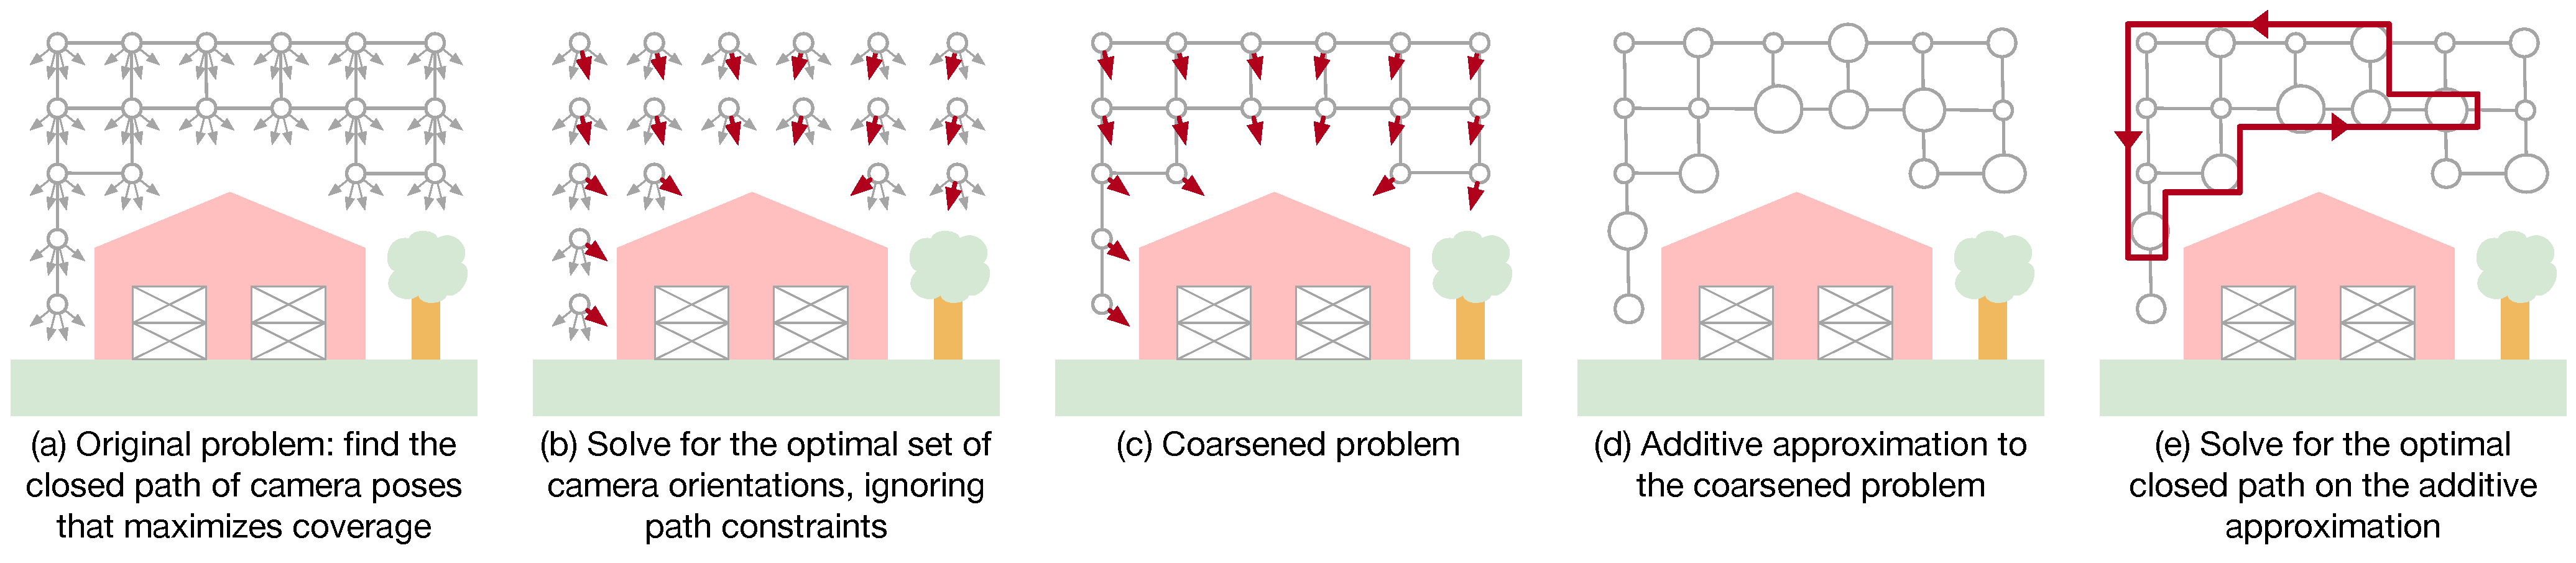
\includegraphics[width=1.0\textwidth]{images/2017_iccv/algorithm_overview.pdf}{\vspace{-10pt}}
\end{center}
\caption{
Overview of our algorithm for generating camera trajectories that maximize coverage.
(a) Our goal is to find the optimal closed path of camera poses through a discrete graph.
(b) We begin by solving for the optimal camera orientation at every node in our graph, ignoring path constraints.
(c) In doing so, we remove the choice of camera orientation from our problem, coarsening our problem into a more standard form.
(d) The solution to the problem in (b) defines an approximation to our coarsened problem, where there is an additive reward for visiting each node.
(e) Finally, we solve for the optimal closed path on the additive approximation defined in (d).
\vspace{-10pt}
}
\label{fig:algorithm_overview}
\end{figure*}

\vspace{-5pt}
\section{Coverage Model for Camera Trajectories}
\label{sec:coverage_model}

In this section, we model the usefulness of a camera trajectory for multi-view stereo reconstruction, in terms of how well it covers the scene geometry.
We provide an overview of our coverage model in Figure \ref{fig:coverage_model}.

In reality, the most useful camera trajectory is the one that yields the highest-quality 3D reconstruction of the scene.
However, it is not clear how we would search for such a camera trajectory directly, without resorting to flying candidate trajectories and performing expensive 3D reconstructions for each of them.
In contrast, our coverage model only roughly approximates the true usefulness of a camera trajectory. 
However, as we will see in the following section, our coverage model: (1) is motivated by established best practices for multi-view stereo image acquisition; (2) is easy to evaluate; (3) only requires a coarse estimate of the scene geometry as input;  and (4) exhibits submodular structure, which will enable us to efficiently maximize it.

\vspace{-10pt}
\paragraph{Best Practices for Multi-View Stereo Image Acquisition}
As a rule of thumb, it is recommended to capture an image every 5--15 degrees around an object, and it is generally accepted that capturing images more densely will eventually lead to diminishing returns in the fidelity of the 3D reconstruction \cite{furukawa:2015}.
Similarly, close-up and fronto-parallel views can help to resolve fine geometric details, because these views increase the effective resolution of estimated depth images, and contribute more reliable texture information to the reconstruction \cite{waechter:2014}.
We explicitly encode these best practices for multi-view stereo image acquisition into our coverage model.

\vspace{-10pt}
\paragraph{Formal Definition}
Given a candidate camera trajectory and approximate scene geometry as a triangle mesh, our goal is to quantify how well the trajectory covers the scene geometry.
We first uniformly sample the camera trajectory to generate a discrete set $C$, consisting of individual camera poses $\mathbf{c}_{0:I}$.
Similarly, we uniformly sample oriented surface points $\mathbf{s}_{0:J}$ from the scene geometry.
For each oriented surface point $\mathbf{s}_j$, we define an oriented hemisphere $H_j$ around it.
For each surface point $\mathbf{s}_j$ and camera $\mathbf{c}_i$, we define a circular disk $D^j_i$ that covers an angular region of the hemisphere $H_j$, centered at the location where $\mathbf{c}_i$ projects onto $H_j$ (see Figure \ref{fig:coverage_model}).
When the surface point $\mathbf{s}_j$ is not visible from the camera $\mathbf{c}_i$, we define the disk $D^j_i$ to have zero radius, and we truncate the extent of each disk so that it does not extend past the equator of $H_j$.
We define the total covered region of the hemisphere $H_j$ as the union of all the disks that partially cover $H_j$ (see Figure \ref{fig:coverage_model}), referring to this total covered region as $V_j = \bigcup_{i=0}^I D^j_i$.
We define our coverage model as follows,
%
\begin{equation}
\begin{aligned}
f(C) = \sum_{j=0}^{J} \int_{V_j} w_j(\mathbf{h}) d\mathbf{h}
\end{aligned}
\label{eqn:model_irregular}
\end{equation}
%
where the outer summation is over all hemispheres; $\int_{V_j} d\mathbf{h}$ refers to the surface integral over the covered region $V_j$; and $w_j(\mathbf{h})$ is a non-negative weight function that assigns different reward values for covering different parts of $H_j$.
Our model can be interpreted as quantifying how well a set of cameras covers the scene's \emph{surface light field} \cite{davis:2012,wood:2000}.
We include a method for efficiently evaluating our coverage model in the supplementary material.

To encourage close-up views, we set the radius of $D^j_i$ to decay exponentially as the camera $\mathbf{c}_i$ moves away from the surface point $\mathbf{s}_j$. To encourage fronto-parallel views, we design each function $w_j(\mathbf{h})$ to decay in a cosine-weighted fashion, as the hemisphere location $\mathbf{h}$ moves away from the hemisphere pole.
We include our exact formulation for $D^j_i$ and $w_j(\mathbf{h})$ in the supplementary material.

\vspace{-10pt}
\paragraph{Submodularity}
Roughly speaking, a set function is submodular if the marginal reward for adding an element to the input set always decreases, as more elements are added to the input set \cite{krause:2014}.
Our coverage model is submodular, because all coverage functions with non-negative weights are submodular \cite{krause:2014}.
Submodularity is a useful property to identify when attempting to optimize a set function, and is often referred to as the discrete analogue of convexity.
We will leverage submodularity extensively in the following section, as we derive our algorithm for generating camera trajectories that maximizing coverage. 

\vspace{-5pt}
\section{Generating Optimal Camera Trajectories}
\label{sec:trajectories}
We provide an overview of our algorithm in Figure \ref{fig:algorithm_overview}.
Our approach is to formulate a reward-collecting optimization problem on a graph.
The nodes in the graph represent camera positions, the edges represent Euclidean distances between camera positions, and the rewards are collected by visiting new nodes.
The goal is to find a path that collects as much reward as possible, subject to a budget constraint on the total path length.
This general problem is known as the \emph{orienteering problem} \cite{gunawan:2016,vansteenwegena:2011}.

A variety of approaches have been proposed to approximately solve the orienteering problem, which is NP-hard.
However, these methods are not directly applicable to our problem, because they assume that the rewards on nodes are additive.
But the total reward we collect in our problem is determined by our coverage model, which does not exhibit additive structure.
Indeed, the marginal reward we collect at a node might be very large, or very small, depending on the entire set of other nodes we visit.


The marginal reward we collect at each node also depends strongly on the orientation of our camera. In other words, our orienteering problem involves extra choices -- how to orient the camera at each visited node -- and these choices are globally coupled through our submodular coverage function. Therefore, even existing algorithms for \emph{submodular orienteering} \cite{chekuri:2012,chekuri:2005,heng:2015,singh:2009a,singh:2009b,zhang:2016} are not directly applicable to our problem, because these algorithms assume there are no extra choices to make at each visited node.

Our strategy will be to apply two successive problem transformations.
First, we leverage submodularity to solve for the approximately optimal camera orientation at every node in our graph, ignoring path constraints (Fig.~\ref{fig:algorithm_overview}b, Section \ref{sec:trajectories_orientation}).
In doing so, we remove the choice of camera orientation from our orienteering problem, thereby coarsening it into a more standard form (Fig.~\ref{fig:algorithm_overview}c).
Second, we leverage submodularity to construct a tight additive approximation of our coverage function (Fig.~\ref{fig:algorithm_overview}d, Section \ref{sec:trajectories_subgradient}).
In doing so, we relax our coarsened submodular orienteering problem into a standard additive orienteering problem.
We formulate this additive orienteering problem as a compact integer linear program, and solve it approximately using a commercially available solver (Fig.~\ref{fig:algorithm_overview}e, Section \ref{sec:trajectories_ilp}).

\vspace{-10pt}
\paragraph{Preprocessing}
We begin by constructing a discrete set of all the possible camera poses we might include in our path.
We refer to this set as our \emph{ground set} of camera poses, $C$.
We construct this set by uniformly sampling a user-defined bounding box that spans the scene, then uniformly sampling a downward-facing unit hemisphere to produce a set of look-at vectors that our drone camera can actuate. We define our ground set as the Cartesian product of these positions and look-at vectors.
We construct the graph for our orienteering problem as the grid graph of all the unique camera positions in $C$, pruned so that it is entirely restricted to the known free space in the scene  (see Section \ref{sec:overview}).

\vspace{-10pt}
\paragraph{Our Submodular Orienteering Problem}
Let $\mathbf{P} = (\mathbf{p}_0, \mathbf{v}_0), (\mathbf{p}_1, \mathbf{v}_1), \ldots, (\mathbf{p}_q, \mathbf{v}_q)$ be a camera path through our graph, represented as a sequence of camera poses taken from our ground set.
We represent each camera pose as a position $\mathbf{p}_i$ and a look-at vector $\mathbf{v}_i$.
We would like to find the optimal path $\mathbf{P}^{\star}$ as follows,
%
\begin{equation}
\begin{aligned}
\mathbf{P}^{\star} = \argmax_{\mathbf{P}} f(C_{\mathbf{P}})~~~~~~~~~~~~~~~~\\
\text{subject to} ~~~~~ l(\mathbf{P}) \leq B ~~~~~ \mathbf{p}_0 = \mathbf{p}_q = \mathbf{p}_\text{root}
\end{aligned}
\label{eqn:submodular_orienteering}
\end{equation}
%
where
$C_\mathbf{P} \subseteq C$ is the set of all the unique camera poses along the path; 
$l(\mathbf{P})$ is the length of the path; $B$ is a user-defined travel budget; and $\mathbf{p}_\text{root}$ is the position where our path must start and end.
For safety reasons, we would also like to design trajectories that consume close to, but no more than, some fixed fraction of our drone's battery (e.g., 80\% or so). However, constraining battery consumption directly is difficult to express in our orienteering formulation, so we model this constraint indirectly by imposing a budget constraint on path length.
We make the observation that our problem is intractable in its current form, because it requires searching over an exponential number of paths through our graph. This observation motivates the following two problem transformations.

\subsection{Solving for Optimal Camera Orientations} 
\label{sec:trajectories_orientation}

Our goal in this subsection is to solve for the optimal camera orientation at every node in our graph, ignoring path constraints. 
We achieve this goal with the following relaxation of the problem in equation (\ref{eqn:submodular_orienteering}).
Let $C_S \subseteq C$ be a subset of camera poses from our ground set. We would like to find the optimal subset of camera poses  $C_S^{\star}$ as follows,
%
\begin{equation}
\begin{aligned}
C_S^{\star} = \argmax_{C_S} f(C_S)~~~~~~~~~\\
\text{subject to} ~~~~~ \left\vert C_S \right\vert = N ~~~~~ C_S \in \mathcal{M}
\end{aligned}
\label{eqn:cardinality_matroid}
\end{equation}
%
where
$\left\vert C_S \right\vert$ is the cardinality of $C_S$;
$N$ is the total number of unique positions in our graph;
and the constraint $C_S \in \mathcal{M}$ enforces mutual exclusion, where we are allowed to select at most one camera orientation at each node in our graph.
In this relaxed problem, we are attempting to maximize coverage by selecting exactly one camera orientation at each node in our graph.
We can interpret such a solution as a coarsened ground set for the problem in equation (\ref{eqn:submodular_orienteering}), thereby transforming it into a standard submodular orienteering problem.

Because our coverage function is submodular, the problem in equation (\ref{eqn:cardinality_matroid}) can be solved very efficiently, and to within 50\% of global optimality, with a very simple greedy algorithm \cite{krause:2014}.
Roughly speaking, the greedy algorithm selects camera poses from our ground set in order of marginal reward, taking care to respect the mutual exclusion constraint, until no more elements can be selected.
Submodularity can also be exploited to significantly reduce the computation time required by the greedy algorithm (e.g., from multiple hours to a couple of minutes, for the problems we consider in this paper) \cite{krause:2014}.
The approximation guarantee in this subsection relies on the fact that selecting more camera poses never reduces coverage, i.e., our coverage function exhibits a property known as \emph{monotonicity} \cite{krause:2014}.
We include a more detailed discussion of the greedy algorithm, and provide pseudocode, in the supplementary material.

\subsection{Additive Approximation of Coverage}
\label{sec:trajectories_subgradient}

Our goal in this subsection is to construct an additive approximation of coverage.
In other words, we would like to define an additive reward at each node in our graph, that closely approximates our coverage function for arbitrary subsets of visited nodes.

To construct our additive approximation, we draw inspiration from the approach of Iyer et al.~\cite{iyer:2013b,iyer:2013a}.
We begin by choosing a permutation of elements in our coarsened ground set.
Let $\mathbf{C} = \mathbf{c}_0, \mathbf{c}_1, \ldots, \mathbf{c}_N$ be our permutation, where $\mathbf{c}_i$ is the $i^{\text{th}}$ element of our coarsened ground set in permuted order.
Let $C_i = \{ \mathbf{c}_0, \mathbf{c}_1, \ldots, \mathbf{c}_{i-1} \}$ be the subset containing the first $i$ elements of our permutation.
We define the additive reward for each element in our permutation as $\tilde{f}_i = f(C_i \cup \mathbf{c}_i) - f(C_i)$.
For an arbitrary subset $C_S$, our additive approximation is simply the sum of additive rewards for each element in $C_S$. Due to submodularity, this additive approximation is guaranteed to be exact for all subsets $C_i$, and to underestimate our true coverage function for all other subsets.
This guarantee is useful for our purposes, because any solution we get from optimizing our additive approximation will yield an equal or greater reward on our true coverage function.

When choosing a permutation, it is generally advantageous to place camera poses with the greatest marginal reward at the front of our permutation.
With this intuition in mind, we form our permutation by sorting the camera poses in our coarsened ground set according to their marginal reward.
Fortunately, we have already computed this ordering in Section \ref{sec:trajectories_orientation} using the greedy algorithm.
So, we simply reuse this ordering to construct our additive approximation.

\subsection{Orienteering as an Integer Linear Program}
\label{sec:trajectories_ilp}

After constructing our additive approximation of coverage, we obtain the following additive orienteering problem, 
%
\begin{equation}
\begin{aligned}
\mathbf{P}^{\star} = \argmax_{\mathbf{P}} \sum_{C_{\mathbf{P}}} \tilde f_i~~~~~~~~~~~~~~~\\
\text{subject to} ~~~~~ l(\mathbf{P}) \leq B ~~~~~ \mathbf{p}_0 = \mathbf{p}_q = \mathbf{p}_\text{root}
\end{aligned}
\label{eqn:ilp}
\end{equation}
%
where $\tilde f_i$ is the additive reward for each unique      node along the path $\mathbf{P}$.
In its current form, it is still not clear how to solve this problem efficiently, because we must still search over an exponential number of paths through our graph.
Fortunately, we can express this problem as a compact integer linear program, using a formulation suggested by Letchford et al.~\cite{letchford:2013}.
We transform our undirected graph into a directed graph, and we define integer variables to represent if nodes are visited and directed edges are traversed.
Remarkably, we can constrain the configuration of these integer variables to form only valid paths through our graph, with a compact set of linear constraints.
We include a more detailed derivation of this formulation in the supplementary material.

Leveraging the formulation suggested by Letchford et al., we convert the problem in equation (\ref{eqn:ilp}) into a standard form that can be given directly to an off-the-shelf solver.
We use the modeling language CVXPY \cite{cvxpy:2016} to specify our problem, and we use the commercially available Gurobi Optimizer \cite{gurobi:2017} as the back-end solver.
Solving integer programming problems to global optimality is NP-hard, and can take a very long time, so we specify a solver time limit of 5 minutes.
Gurobi returns the best feasible solution it finds within the time limit, along with a worst-case optimality gap.
In our experience, Gurobi consistently converges to a close-to-optimal solution in the allotted time (i.e., typically with an optimality gap of less than 10\%).
At this point, the resulting orienteering trajectory can be safely and autonomously executed on our drone.

%%MOVE THIS TO APPENDIX
%We replace each undirected edge in our graph with two directed \emph{arcs}, each with the same cost as the original undirected edge.
%We define the indicator vectors $\mathbf{x}$ and $\mathbf{y}$ to represent whether or not each arc is traversed and
%whether or not each node in our graph is visited respectively. Also let vector $\mathbf{g}$ contain the cumulative costs incurred so far, when beginning to traverse each arc. Finally, we define the constant vector $\mathbf{f}$ to contain the additive reward at each each node, and a constant vector $\mathbf{r}$ to contain the instantaneous cost of traversing each arc.

%We also define inbound and outbound \emph{node-arc indicator matrices}, $\mathbf{A}^{\text{in}}$ and $\mathbf{A}^{\text{out}}$ respectively. The rows of these matrices represent the nodes in our graph, and columns represent the arcs.
%We set the entry of $\mathbf{A}^{\text{in}}$ corresponding to \{node $n$, arc $m$\} equal to 1 if arc $m$ is an inbound arc for node $n$, and equal to 0 otherwise. We define $\mathbf{A}^{\text{out}}$ similarly, but with respect to the outbound arcs.
%We use the notation $\mathbf{A}_{R}$ to refer to the row of $\mathbf{A}$ corresponding to the root node (i.e., the node where our path must start and end), and we use the notation $\mathbf{A}_{R'}$ to refer to all the other rows of $\mathbf{A}$. We define our integer linear program as follows:
%
%\begin{subequations}
%\label{eqn:ilp}
%\begin{equation}
%\begin{aligned}
%\mathbf{x}^{\star}, \mathbf{y}^{\star}, \mathbf{g}^{\star} = \argmax_{ \mathbf{x}, \mathbf{y}, \mathbf{g} } \mathbf{f}^T \mathbf{y}
%\end{aligned}
%\label{eqn:ilp_a}
%\end{equation}
%
%\vspace{-5pt}
%
%\begin{equation}
%\begin{aligned}
%\text{subject to} ~~~~~ \mathbf{r}^T \mathbf{x} \leq b
%\end{aligned}
%\label{eqn:ilp_b}
%\end{equation}
%
%\vspace{-5pt}
%
%\begin{equation}
%\begin{aligned}
%\mathbf{A}^{\text{out}}_{R}  \mathbf{x} & \geq \mathbf{1}             &     \mathbf{A}^{\text{out}}      \mathbf{x}                                          & = \mathbf{A}^{\text{in}}      \mathbf{x} \\
%\mathbf{A}^{\text{out}}_{R'} \mathbf{x} & \geq \mathbf{y}_{R'} ~~~~~~ &     \mathbf{A}^{\text{out}}_{R'} \mathbf{g} - \mathbf{A}^{\text{in}}_{R'} \mathbf{g} & = \mathbf{A}^{\text{in}}_{R'} \mathbf{T} \mathbf{x} \\
%\end{aligned}
%\label{eqn:ilp_c}
%\end{equation}
%
%\vspace{-4pt}
%
%\begin{equation}
%\begin{aligned}
%0 \leq \mathbf{g} \leq \mathbf{U} \mathbf{x}\\
%\end{aligned}
%\label{eqn:ilp_d}
%\end{equation}
%
%\vspace{-10pt}
%
%\begin{equation}
%\begin{aligned}
%\mathbf{x} \in \{0,1\}^M ~~~~~ \mathbf{y} \in \{0,1\}^N ~~~~~ \mathbf{g} \in \mathbf{R}_{+}^M
%\end{aligned}
%\label{eqn:ilp_e}
%\end{equation}
%\end{subequations}
%
%where
%the matrix $\mathbf{T} = \mathbf{diag}( \mathbf{r} )$ helps us to calculate an intermediate matrix of instantaneous costs for inbound arcs;
%the matrix $\mathbf{U} = \mathbf{diag}( \mathbf{1}b - \mathbf{r} )$ helps us to define the upper bounds for our cumulative cost variable $\mathbf{g}$;
%and $M$ is the number of arcs in our graph and $N$ is the number of nodes.
%In this formulation, $\mathbf{x}$, $\mathbf{y}$, and $\mathbf{g}$ are decision variables, everything else is problem data.

%The objective in this optimization problem (\ref{eqn:ilp_a}) attempts to maximize the reward we collect, by activating as many nodes as possible. The constraint in (\ref{eqn:ilp_b}) enforces our maximum budget on total path length.
%The constraints in (\ref{eqn:ilp_c}) specify that: at least one of the outbound arcs for the root node must be active; the number of active outbound arcs must match the number of active inbound arcs at each node; if an outbound arc is active, then the node at its tail must be active; and the difference in cumulative cost at an outbound arc and a corresponding inbound arc, must match the instantaneous cost of the inbound arc.
%The constraint in (\ref{eqn:ilp_d}) enforces that the cumulative costs incurred so far are less than the total budget.
%Finally, the constraints in (\ref{eqn:ilp_e}) specify that $\mathbf{x}$ and $\mathbf{y}$ are Boolean indicator vectors, and that $\mathbf{g}$ is non-negative and real-valued.

%The problem in equation (\ref{eqn:ilp}) is in a standard form. 
